\documentclass[tikz,border=10pt]{standalone}
\usetikzlibrary{arrows.meta, positioning, calc, decorations.pathreplacing}
\usepackage{amssymb}

\begin{document}
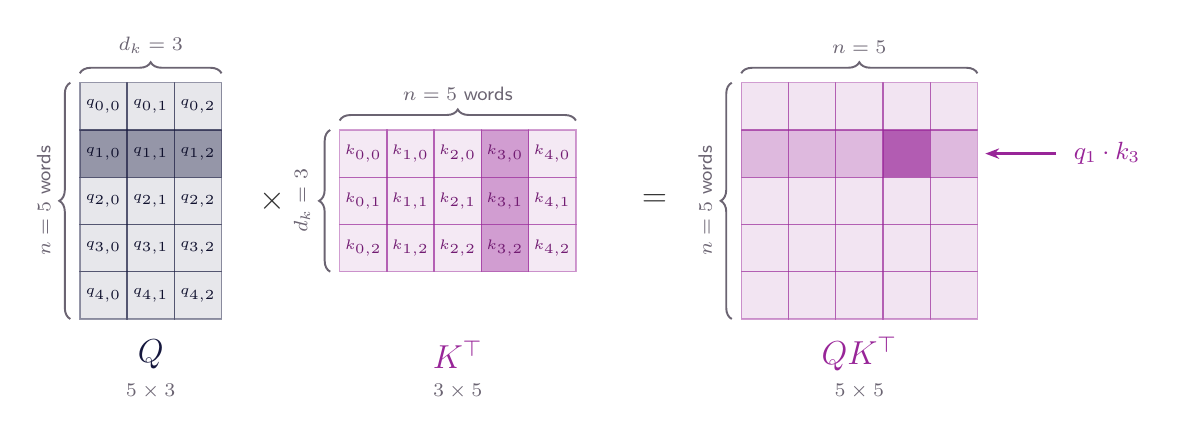
\begin{tikzpicture}[
    every node/.style={font=\sffamily},
]

\definecolor{c1}{HTML}{15173D}   % queries
\definecolor{c2}{HTML}{982598}   % keys, and the scores they produce
\definecolor{c3}{HTML}{E491C9}
\definecolor{c4}{HTML}{F1E9E9}
\definecolor{axiscolor}{HTML}{333333}
\definecolor{labelcolor}{HTML}{6B6472}

\def\cs{0.6}     % cell size

% ================================================================
%   Q        top-left (0, 4.2)     5 rows x 3 cols
%   K^T      top-left (3.3, 3.6)   3 rows x 5 cols
%   QK^T     top-left (8.4, 4.2)   5 rows x 5 cols
%   the highlighted pair: row 1 of Q, column 3 of K^T (zero-based)
% ================================================================

% ---------------------------------------------------------------- Q
\foreach \r in {0,...,4} {
    \foreach \c in {0,1,2} {
        \pgfmathsetmacro{\op}{ifthenelse(\r==1, 0.45, 0.10)}
        \fill[c1, opacity=\op] (\c*\cs, 4.2-\r*\cs-\cs) rectangle ++(\cs, \cs);
        \draw[c1, opacity=0.45, line width=0.5pt]
            (\c*\cs, 4.2-\r*\cs-\cs) rectangle ++(\cs, \cs);
        \node[font=\sffamily\tiny, text=c1!75!black]
            at (\c*\cs+0.5*\cs, 4.2-\r*\cs-0.5*\cs) {$q_{\r,\c}$};
    }
}
\node[font=\sffamily\large, text=c1] at (0.9, 0.75) {$Q$};
\node[font=\sffamily\scriptsize, text=labelcolor] at (0.9, 0.28) {$5 \times 3$};

\draw[decorate, decoration={brace, amplitude=4pt}, labelcolor, line width=0.7pt]
    (0, 4.32) -- (1.8, 4.32);
\node[font=\sffamily\scriptsize, text=labelcolor, anchor=south] at (0.9, 4.45)
    {$d_k = 3$};
\draw[decorate, decoration={brace, amplitude=4pt}, labelcolor, line width=0.7pt]
    (-0.12, 1.2) -- (-0.12, 4.2);
\node[font=\sffamily\scriptsize, text=labelcolor, anchor=south, rotate=90]
    at (-0.25, 2.7) {$n = 5$ words};

\node[font=\sffamily\large, text=axiscolor] at (2.45, 2.7) {$\times$};

% ---------------------------------------------------------------- K transpose
\foreach \r in {0,1,2} {
    \foreach \c in {0,...,4} {
        \pgfmathsetmacro{\op}{ifthenelse(\c==3, 0.45, 0.10)}
        \fill[c2, opacity=\op] (3.3+\c*\cs, 3.6-\r*\cs-\cs) rectangle ++(\cs, \cs);
        \draw[c2, opacity=0.45, line width=0.5pt]
            (3.3+\c*\cs, 3.6-\r*\cs-\cs) rectangle ++(\cs, \cs);
        \node[font=\sffamily\tiny, text=c2!75!black]
            at (3.3+\c*\cs+0.5*\cs, 3.6-\r*\cs-0.5*\cs) {$k_{\c,\r}$};
    }
}
\node[font=\sffamily\large, text=c2] at (4.8, 0.75) {$K^{\top}$};
\node[font=\sffamily\scriptsize, text=labelcolor] at (4.8, 0.28) {$3 \times 5$};

\draw[decorate, decoration={brace, amplitude=4pt}, labelcolor, line width=0.7pt]
    (3.3, 3.72) -- (6.3, 3.72);
\node[font=\sffamily\scriptsize, text=labelcolor, anchor=south] at (4.8, 3.85)
    {$n = 5$ words};
\draw[decorate, decoration={brace, amplitude=4pt}, labelcolor, line width=0.7pt]
    (3.18, 1.8) -- (3.18, 3.6);
\node[font=\sffamily\scriptsize, text=labelcolor, anchor=south, rotate=90]
    at (3.05, 2.7) {$d_k = 3$};

\node[font=\sffamily\large, text=axiscolor] at (7.3, 2.7) {$=$};

% ---------------------------------------------------------------- QK^T
\foreach \r in {0,...,4} {
    \foreach \c in {0,...,4} {
        % the whole of row 2 is shaded, since that row is one word's five
        % scores; the single darker cell inside it is where column 4 met it
        \pgfmathsetmacro{\op}{ifthenelse(\r==1 && \c==3, 0.75,
                                        ifthenelse(\r==1, 0.32, 0.12))}
        \fill[c2, opacity=\op] (8.4+\c*\cs, 4.2-\r*\cs-\cs) rectangle ++(\cs, \cs);
        \draw[c2, opacity=0.45, line width=0.5pt]
            (8.4+\c*\cs, 4.2-\r*\cs-\cs) rectangle ++(\cs, \cs);
    }
}
\draw[decorate, decoration={brace, amplitude=4pt}, labelcolor, line width=0.7pt]
    (8.28, 1.2) -- (8.28, 4.2);
\node[font=\sffamily\scriptsize, text=labelcolor, anchor=south, rotate=90]
    at (8.15, 2.7) {$n = 5$ words};

\node[font=\sffamily\large, text=c2] at (9.9, 0.75) {$QK^{\top}$};
\node[font=\sffamily\scriptsize, text=labelcolor] at (9.9, 0.28) {$5 \times 5$};

\draw[decorate, decoration={brace, amplitude=4pt}, labelcolor, line width=0.7pt]
    (8.4, 4.32) -- (11.4, 4.32);
\node[font=\sffamily\scriptsize, text=labelcolor, anchor=south] at (9.9, 4.45)
    {$n = 5$};

% ---------------------------------------------------------------- one entry
\draw[-{Stealth[length=5pt]}, line width=1.0pt, c2]
    (12.4, 3.3) -- (11.5, 3.3);
\node[font=\sffamily\small, text=c2, anchor=west] at (12.5, 3.3)
    {$q_1 \cdot k_3$};

\end{tikzpicture}
\end{document}
